\section{Multiply and divide}
\label{sec:muldiv}

The M extension has eight instructions. All use opcode OP with funct7 = \texttt{0000001}. funct3 selects the instruction (Table~\ref{tab:mmap}).

\begin{guidetable}{The M extension map}{mmap}{c l l l}
funct3 & instruction & operands & result \\
\midrule
\texttt{000} & MUL    & either & low 32 bits of the product \\
\texttt{001} & MULH   & signed $\times$ signed & high 32 bits \\
\texttt{010} & MULHSU & signed $\times$ unsigned & high 32 bits \\
\texttt{011} & MULHU  & unsigned $\times$ unsigned & high 32 bits \\
\texttt{100} & DIV    & signed & quotient \\
\texttt{101} & DIVU   & unsigned & quotient \\
\texttt{110} & REM    & signed & remainder \\
\texttt{111} & REMU   & unsigned & remainder \\
\end{guidetable}

\subsection{Multiply}

The Cyclone II multipliers are 18 $\times$ 18 bits, signed. A 32-bit multiply needs four of them.

First, EX extends each operand to 33 bits. A signed operand gets a copy of its sign bit. An unsigned operand gets a 0. All four multiply instructions then use one signed $33 \times 33$ multiplier, and the result is 66 bits.

Each 33-bit operand has a signed high part of 17 bits and an unsigned low part of 16 bits:
\begin{equation*}
  a = a_H \cdot 2^{16} + a_L, \qquad -2^{16} \le a_H < 2^{16}, \quad 0 \le a_L < 2^{16} .
\end{equation*}
The product is the sum of four partial products (Figure~\ref{fig:pp}):
\begin{equation*}
  a\,b = a_H b_H \cdot 2^{32} + (a_H b_L + a_L b_H) \cdot 2^{16} + a_L b_L .
\end{equation*}

\begin{figure}[H]
  \centering
  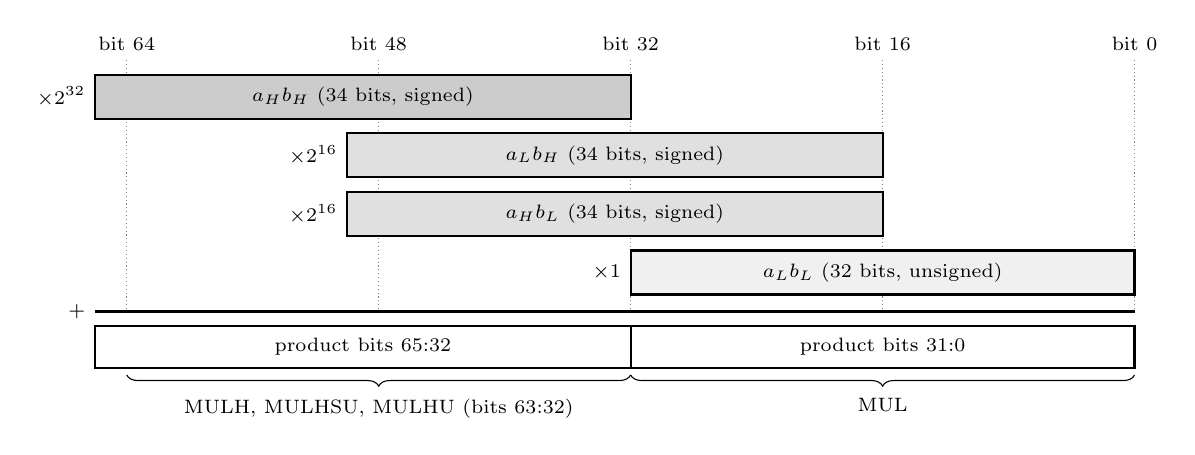
\begin{tikzpicture}[x=0.2cm, y=0.62cm, font=\scriptsize]
    \foreach \b in {0,16,32,48,64} {
      \node[above] at ({66-\b},4.9) {bit \b};
      \draw[gray, densely dotted] ({66-\b},4.9) -- ({66-\b},-0.25);}
    \draw[thick, fill=black!20] (0,3.7) rectangle (34,4.6);           \node at (17,4.15) {$a_H b_H$ (34 bits, signed)};
    \draw[thick, fill=black!12] (16,2.5) rectangle (50,3.4);          \node at (33,2.95) {$a_L b_H$ (34 bits, signed)};
    \draw[thick, fill=black!12] (16,1.3) rectangle (50,2.2);          \node at (33,1.75) {$a_H b_L$ (34 bits, signed)};
    \draw[thick, fill=black!6]  (34,0.1) rectangle (66,1.0);          \node at (50,0.55) {$a_L b_L$ (32 bits, unsigned)};
    \node[left] at (0,4.15) {$\times 2^{32}$};
    \node[left] at (16,2.95) {$\times 2^{16}$};
    \node[left] at (16,1.75) {$\times 2^{16}$};
    \node[left] at (34,0.55) {$\times 1$};
    \draw[very thick] (0,-0.25) -- (66,-0.25);
    \node[left] at (0,-0.25) {$+$};
    \draw[thick] (0,-1.4) rectangle (66,-0.55);
    \draw[thick] (34,-1.4) -- (34,-0.55);
    \node at (17,-0.975) {product bits 65:32};
    \node at (50,-0.975) {product bits 31:0};
    \draw[decorate, decoration={brace, mirror, amplitude=4pt}] (34,-1.55) -- (66,-1.55) node[midway, below=5pt] {MUL};
    \draw[decorate, decoration={brace, mirror, amplitude=4pt}] (2,-1.55) -- (34,-1.55) node[midway, below=5pt] {MULH, MULHSU, MULHU (bits 63:32)};
  \end{tikzpicture}
  \caption{The four partial products of a $33 \times 33$ signed multiply}
  \label{fig:pp}
\end{figure}

A multiply uses four cycles in EX:

\begin{enumerate}
  \item \texttt{X\_RUN}: extend the operands into \texttt{mul\_a} and \texttt{mul\_b}.
  \item \texttt{X\_MUL0}: calculate the four partial products. Each has a register.
  \item \texttt{X\_MUL1}: shift and add the partial products into \texttt{mul\_p}.
  \item \texttt{X\_MUL2}: select bits 31:0 (MUL) or bits 63:32 (MULH, MULHSU, MULHU).
\end{enumerate}

The registers between the steps keep each step shorter than the 20 ns clock period.

\subsection{Divide}

The divider uses the restoring algorithm and calculates one quotient bit in each cycle. It operates on unsigned values:

\begin{itemize}
  \item For DIV and REM, the divider first makes the two operands positive.
  \item The quotient is negative if the operand signs are different.
  \item The remainder has the sign of the dividend.
\end{itemize}

The register \texttt{div\_quo} holds the dividend at the start. In each cycle, the top bit of \texttt{div\_quo} shifts into the remainder, and the new quotient bit shifts into the bottom of \texttt{div\_quo}. After 32 cycles, \texttt{div\_quo} holds the quotient. Figure~\ref{fig:divflow} shows one cycle.

\begin{figure}[H]
  \centering
  \begin{tikzpicture}[node distance=0.55cm]
    \node[box] (s0) {\texttt{rem2} $\leftarrow$ \{\texttt{rem[30:0]}, \texttt{quo[31]}\}};
    \node[box, below=of s0] (s1) {\texttt{diff} $\leftarrow$ \texttt{rem2} $-$ \texttt{den} \quad (33 bits)};
    \node[decision, below=of s1] (d) {\texttt{rem[31]} = 1\\or \texttt{diff} $\ge 0$?};
    \node[box, below left=0.6cm and 0.2cm of d] (y) {\texttt{rem} $\leftarrow$ \texttt{diff}\\\texttt{quo} $\leftarrow$ \{\texttt{quo[30:0]}, 1\}};
    \node[box, below right=0.6cm and 0.2cm of d] (n) {\texttt{rem} $\leftarrow$ \texttt{rem2}\\\texttt{quo} $\leftarrow$ \{\texttt{quo[30:0]}, 0\}};
    \node[box, below=1.9cm of d] (c) {\texttt{count} $\leftarrow$ \texttt{count} $-$ 1};
    \draw[tr] (s0) -- (s1);
    \draw[tr] (s1) -- (d);
    \draw[tr] (d) -| node[cond, above, pos=0.25] {yes} (y);
    \draw[tr] (d) -| node[cond, above, pos=0.25] {no} (n);
    \draw[tr] (y) |- (c);
    \draw[tr] (n) |- (c);
  \end{tikzpicture}
  \caption{One cycle of the divider in \texttt{X\_DIV}}
  \label{fig:divflow}
\end{figure}

The test of \texttt{rem[31]} is for a divisor of $2^{31}$ or more. If \texttt{rem[31]} is 1, the shifted remainder is a 33-bit value and is larger than the divisor. The divider must subtract, although the 33-bit \texttt{diff} has lost the top bit.

Table~\ref{tab:divex} shows the algorithm for 4-bit operands. The CPU uses 32 bits and 32 steps.

\begin{guidetable}{Restoring division, 4-bit example: $13 \div 3 = 4$ remainder 1}{divex}{c c c c c c}
step & rem before & quo before & shifted rem & rem $-$ 3 & result bit \\
\midrule
1 & 0000 & 1101 & 0001 & $-2$ & 0 \\
2 & 0001 & 1010 & 0011 & 0    & 1 \\
3 & 0000 & 0101 & 0000 & $-3$ & 0 \\
4 & 0000 & 1010 & 0001 & $-2$ & 0 \\
\midrule
\multicolumn{6}{l}{after step 4 the quotient register reads \texttt{0100} = 4, the remainder \texttt{0001} = 1} \\
\end{guidetable}

RISC-V defines the result of each division, and no division causes a trap. The divider detects the two special cases at the start (Table~\ref{tab:divspecial}).

\begin{guidetable}{Division special cases}{divspecial}{l l l}
case & quotient & remainder \\
\midrule
divide by zero & all ones ($-1$, or $2^{32}-1$) & the dividend \\
$-2^{31} \div -1$ (signed overflow) & $-2^{31}$ & 0 \\
\end{guidetable}

A divide uses 34 cycles in EX: one to load the operands, 32 steps, and one to select the result.
